% 固定来源PDF印刷页52第22题正三棱柱及截面的示意重绘。
% E位于BB1中点；透视尺寸仅用于表示点线关系，不作为度量条件。
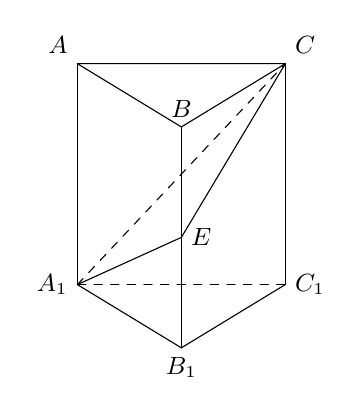
\begin{tikzpicture}[scale=1.1,line join=round,line cap=round,
  every node/.style={font=\small}]
\coordinate (A) at (0,2.55);
\coordinate (B) at (1.2,1.82);
\coordinate (C) at (2.4,2.55);
\coordinate (Aone) at (0,0);
\coordinate (Bone) at (1.2,-.73);
\coordinate (Cone) at (2.4,0);
\coordinate (E) at (1.2,.545);
% Two triangular bases and the connecting edges.
\draw (A)--(B)--(C)--cycle;
\draw (A)--(Aone) (B)--(Bone) (C)--(Cone);
\draw (Aone)--(Bone)--(Cone);
\draw[dashed] (Aone)--(Cone);
% Cross-section A1EC; A1C and the hidden base edge are dashed in the source.
\draw (Aone)--(E)--(C);
\draw[dashed] (Aone)--(C);
\node[above left] at (A) {$A$};
\node[above] at (B) {$B$};
\node[above right] at (C) {$C$};
\node[left] at (Aone) {$A_1$};
\node[below] at (Bone) {$B_1$};
\node[right] at (Cone) {$C_1$};
\node[right] at (E) {$E$};
\end{tikzpicture}
